\chapter{\label{results}Results and Discussion}
After implementing the code, the filter can be generated as per user's requirements. Some plots are included with did not use the filter but represent the results which are obtained by stacking the void galaxies. MILCA refers to Modified Internal Linear Component Algorithm (\cite{hurier_milca_2013}), which is a internal linear combination (ILC) method used to extract the CMB emission from the WMAP multifrequency data courtesy projects like the Planck survey. NILC stands for Needlet Internal Linear Combination (\cite{remazeilles_cmb_2011}), a different technique used for same purpose.
\begin{figure}[h!]
	\centering
	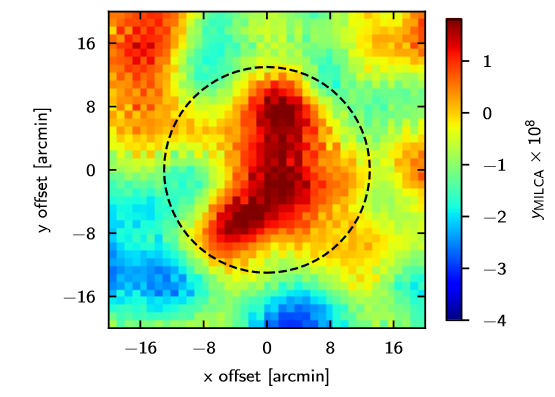
\includegraphics{fig2.png}
	\caption{The normalized stacked $ y $ MILCA map at void galaxy locations at all z in our sample over $ 51\% $ sky mask.}
\end{figure}
\begin{figure}[h!]
	\centering
	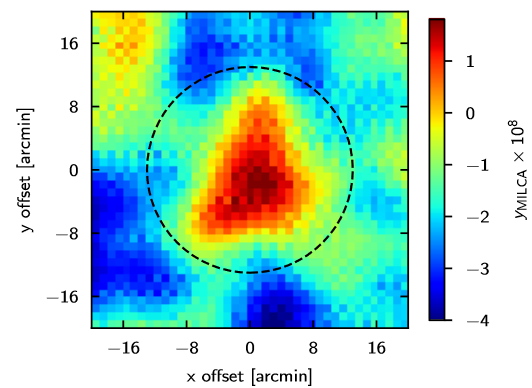
\includegraphics{fig3-1.png}
	\caption{The normalized stacked $ y $ MILCA map at void galaxy locations at $ z > 0.04 $ in our sample over $ 51\% $ sky mask.}
\end{figure}
\begin{figure}[h!]
	\centering
	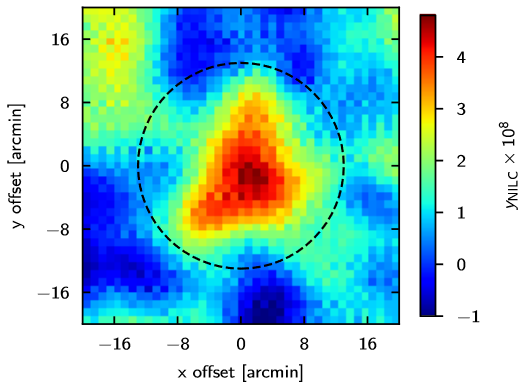
\includegraphics{fig3-2.png}
	\caption{The normalized stacked $ y $ NILC map at void galaxy locations at $ z > 0.04 $ in our sample over $ 51\% $ sky mask.}
\end{figure}
Using the filter, similar stacking plots can be obtained. The filtering will aid in removing unwanted galaxies, that are too near the void walls. 
\setcounter{equation}{0}
\setcounter{table}{0}
\setcounter{figure}{0}
%\baselineskip 24pt


    



